% To compile:
% pdflatex Writeup.tex

% ==============================================================
% Latex packages and settings
% ==============================================================
\documentclass[11pt]{article}

% Language setting:
% Replace `english' with e.g. `spanish' to change the document language
\usepackage[english]{babel}                             % Set document language (hyphenation, date formats, etc.)

% Set caption formatting:
\usepackage{caption}                                    % Control the appearance of figure and table captions
\captionsetup[table]{labelfont=bf, font=small}          % Make table labels bold and use a small font for table captions
\captionsetup[figure]{labelfont=bf, font=small}         % Make figure labels bold and use a small font for figure captions

\usepackage{subcaption}                                 % Allow subFigures_compressed/subtables with individual sub-captions

% Set page size and margins:
% Replace `letterpaper' with `a4paper' for UK/EU standard size
\usepackage[a4paper,top=2cm,bottom=2cm,left=2.5cm,right=2.5cm,marginparwidth=1.75cm]{geometry} % Configure paper size and margins

% Useful packages
\usepackage{amsmath}                                    % Enhanced math environments and symbols
\usepackage{amssymb}                                    % Additional math symbols
\usepackage{graphicx}                                   % Include and scale external graphics (e.g. .pdf, .png)
\usepackage[colorlinks=true,                            % Use colored links instead of boxed links
            allcolors=blue,                             % Use blue for all link types (cite, ref, url)
            bookmarksnumbered=true,                     % Number the PDF bookmarks according to section numbers
            bookmarksopen=true,                         % Open the bookmark tree when the PDF is opened
            bookmarksopenlevel=10]{hyperref}            % Control depth to which bookmarks are expanded
\usepackage{listings}                                   % Typeset source code with syntax highlighting

\usepackage{authblk}                                    % Manage authors and affiliations in a structured way
% Make only the author and/or affiliation smaller
\renewcommand\Authfont{\small}                        % Set the Author font size (e.g. small or footnotesize)
\renewcommand\Affilfont{\small}                         % Set the affiliation font size (e.g. small or footnotesize)
\renewcommand\Authand{}        % <-- add this

\usepackage{comment}                                    % Define large comment environments to exclude blocks from output
\usepackage{enumitem}                                   % Customize list environments (itemize, enumerate, etc.)
\usepackage{lineno}                                     % Add optional line numbers to the document
% \usepackage[backend=biber, style=numeric-comp, citestyle=numeric-comp, sorting=none]{biblatex} % Modern bibliography management with biber backend
\usepackage[backend=biber, sorting=none, style=numeric, citestyle=numeric]{biblatex} % Modern bibliography management with biber backend
\addbibresource{references.bib}                    % Load bibliography entries for citations and references
% Make bibliography font smaller
\renewcommand*{\bibfont}{\footnotesize}                 % Reduce font size in the bibliography
\usepackage{multirow}                                   % Enable table cells that span multiple rows
\usepackage{rotating}                                   % Rotate figures, tables, or text (e.g. sideways tables)
\usepackage{pdfpages}                                   % Include external PDF pages in the document
\usepackage{csquotes}                                   % Context-sensitive quotation marks, recommended with biblatex
\usepackage[table]{xcolor}                              % Color support, including coloring table rows/columns
\usepackage{array, makecell, colortbl}                  % Extra tools for tables: new column types, multi-line cells, colored cells
\renewcommand{\arraystretch}{1.5}                       % Increase row height in tables by a factor of 1.5
% \setlength{\parskip}{1\baselineskip}                    % Adds a full line space between paragraphs
\setlength{\parindent}{0pt}                             % Optional: removes paragraph indentation

\usepackage{sidecap}

% ==============================================================
% Document title and author
% ==============================================================
\title{\textbf{Numerical Methods in Astrophysics (0321488101): Numerov Method for Bound States in the One-Dimensional Schr\"odinger Equation}}
\author{Alon Sportes (ID: 204498745)}
\date{}

% ==============================================================
% Document content
% ==============================================================
\begin{document}
    \maketitle

    \vfill

    \phantomsection
    \begingroup
        \setlength{\parskip}{0pt}
        \addcontentsline{toc}{section}{Table of Contents}
        \tableofcontents
    \endgroup
    \vfill

    % Start citation tracking here
    \begin{refsection}

    \newpage

    % ==============================================================
    % Introduction
    % ==============================================================
    \section{Introduction}
        This project studies the one-dimensional time-independent Schr\"odinger equation using the Numerov method combined with parity-aware shooting. The aim is to validate the method on problems with known analytic spectra, quantify its numerical accuracy, and then apply it to more interesting bound-state potentials such as a double well and a finite square well. Scattering from finite barriers is included as a secondary extension. \\

        This is a boundary-value eigenvalue problem rather than a standard initial-value problem: only special energies satisfy the required boundary behavior. Numerov is well suited to this task because the equation has the second-order form $\psi''=q(x)\psi$ with no first-derivative term. The project therefore emphasizes both the computed spectra and the numerical checks behind them, including analytic benchmarks, convergence studies, parity and node structure, and probability conservation in the scattering extension. \\
        
        The full Python implementation is available in \href{https://github.com/alons126/Numerov-bound-states}{this repository}. The accompanying \href{https://github.com/alons126/Numerov-bound-states/blob/main/README.md}{\texttt{README.md}} and documentation describe how to run the code and reproduce the results.

    % ==============================================================
    % Computational approach
    % ==============================================================
    \section{Computational approach}
        \subsection{The Schr\"odinger equation and Numerov method}
            In dimensionless units, the Schr\"odinger equation is written as:
            \begin{equation}
            \psi''(x) = 2\,[V(x)-E]\psi(x)
            \end{equation}
            The wavefunction is integrated with the Numerov scheme on a uniform grid. For the symmetric bound-state potentials studied here, $V(-x)=V(x)$, so the eigenstates can be chosen to have definite parity: even states satisfy $\psi'(0)=0$ and odd states satisfy $\psi(0)=0$. This symmetry lets the solver work only on the half-domain $[0,x_{\max}]$ and reconstruct the other half by reflection. Eigenvalues are then obtained by searching for zeros of a scalar mismatch function and refining the resulting brackets with robust root finding. The implementation follows the standard Numerov-shooting strategy described in \cite{Pang_2006}.

        \subsection{Shooting and root finding}
            The boundary-value problem is reformulated as a root-finding problem for a mismatch function $M(E)$. For a trial energy $E$, the Schr\"odinger equation is integrated and a boundary mismatch is evaluated. The code uses two related formulations. For the infinite square well, finite square well, and quartic double well, the solution is shot outward from $x=0$ and the mismatch is the boundary value $M(E)=\psi_E(x_{\max})$. For the harmonic oscillator and the RK4 comparison, the integration is instead started from the decaying tail at $x_{\max}$ and the parity condition is enforced at the origin:
            \begin{align}
            \text{even states:}\quad M(E) = \psi'_E(0),\,\,\,\,\,\,\,\,\,\,\text{odd states:}\quad M(E) = \psi_E(0)
            \end{align}
            The inward formulation is specialized to smooth confining problems where the truncation point already lies in a forbidden decaying region. In all cases, eigenvalues correspond to roots of $M(E)=0$, found by bracketing sign changes and then refining them numerically using standard root-finding ideas \cite{Pang_2006}. The outward solver uses bisection followed by a short safeguarded polishing step inside the final bracket, while the inward and RK4 solvers use straight bisection. In the inward even-state case, $\psi'(0)$ is evaluated with a fourth-order backward stencil so the boundary condition does not reduce the overall observed order of accuracy.

    % ==============================================================
    % Results
    % ==============================================================
    \section{Results}
        Each potential is used to validate, test, or demonstrate different aspects of the numerical method, ranging from analytic benchmarks to nontrivial quantum behavior.

        \subsection{Infinite square well}
            \begin{figure}[!b]
                \centering
                
                \begin{minipage}[t]{0.48\textwidth}
                    \centering
                    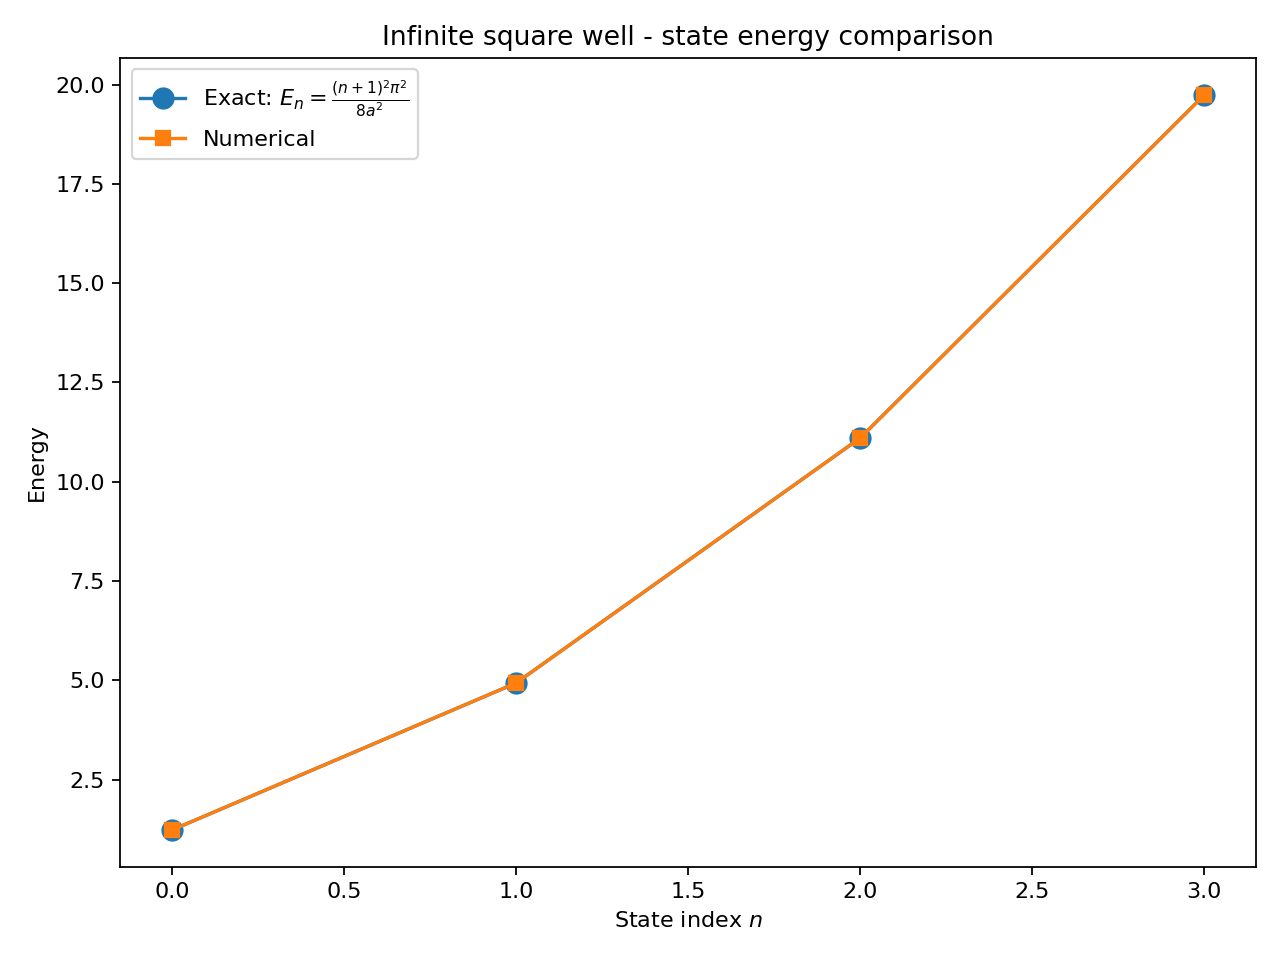
\includegraphics[width=\textwidth]{../../results/1_infinite_square_well_Numerov/1_infinite_square_well_Numerov_state_energy_comparison.png}
                    \captionof{figure}{Numerical and exact energy eigenvalues for the infinite square well.}
                    \label{fig:infwell_energies}
                \end{minipage}
                \hfill
                \begin{minipage}[t]{0.48\textwidth}
                    \centering
                    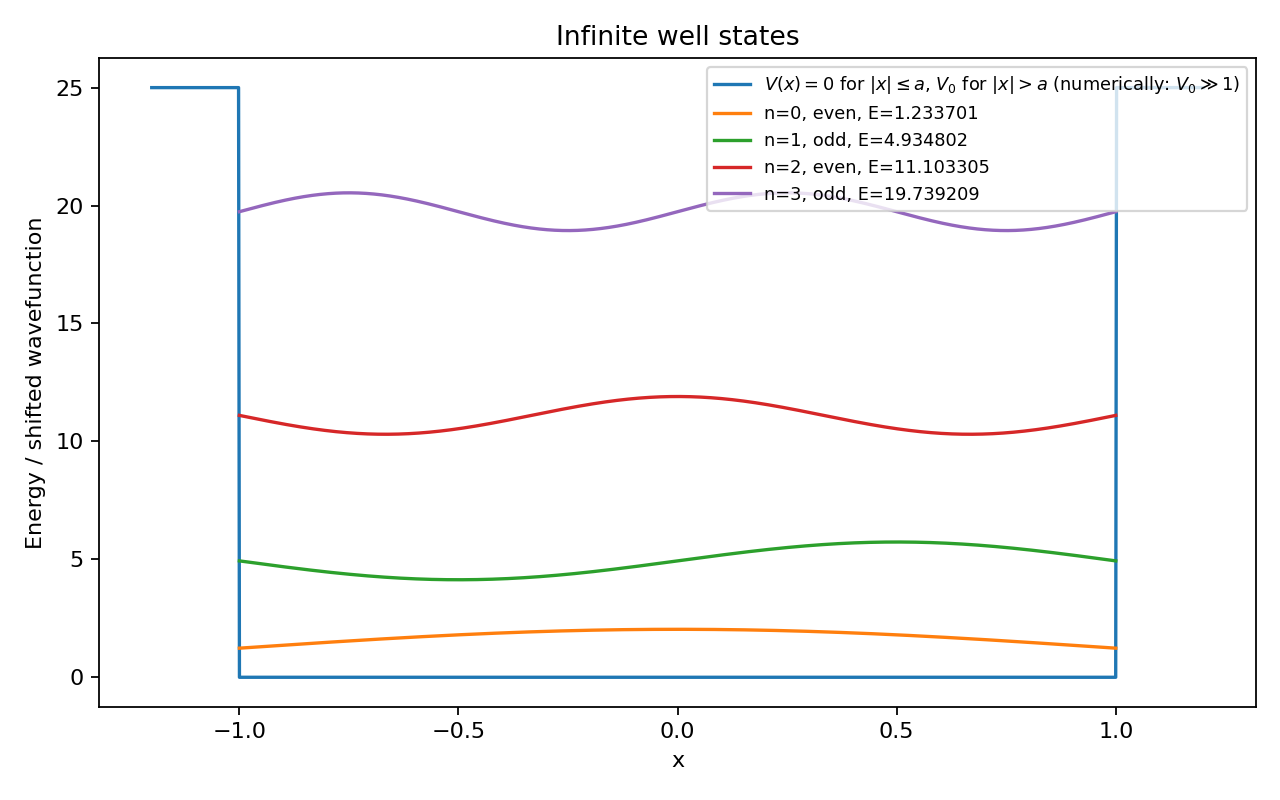
\includegraphics[width=\textwidth]{../../results/1_infinite_square_well_Numerov/1_infinite_square_well_Numerov_states.png}
                    \captionof{figure}{Wavefunctions for the first four infinite-square-well states.}
                    \label{fig:infwell_states}
                \end{minipage}

                \vspace{1em}

                \begin{minipage}[t]{\textwidth}
                    \centering
                    \begin{subfigure}[t]{0.485\textwidth}
                        \centering
                        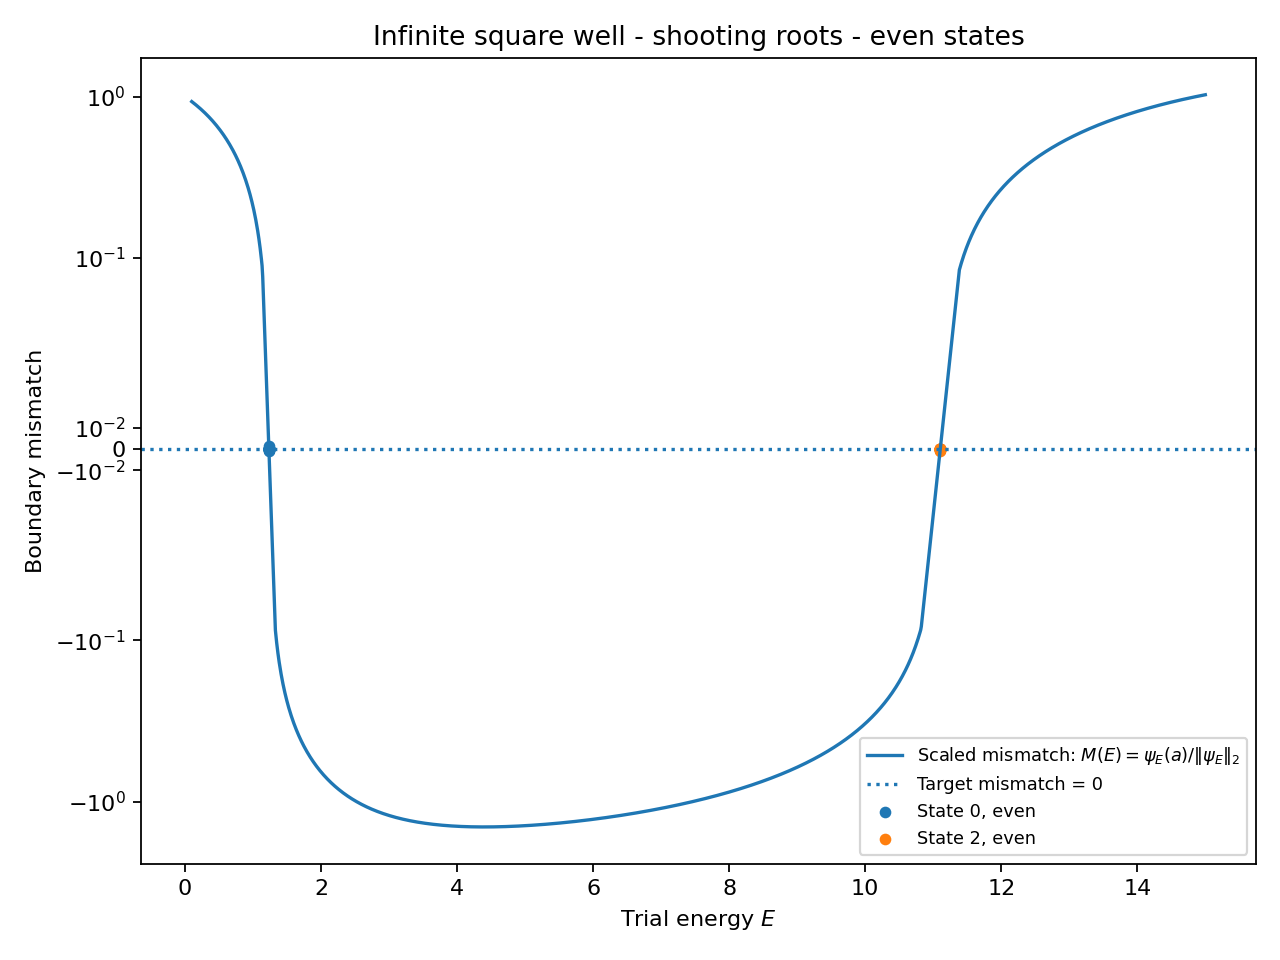
\includegraphics[height=5cm]{../../results/1_infinite_square_well_Numerov/1_infinite_square_well_Numerov_root_finding_even.png}
                        \caption{}
                    \end{subfigure}
                    \hfill
                    \begin{subfigure}[t]{0.485\textwidth}
                        \centering
                        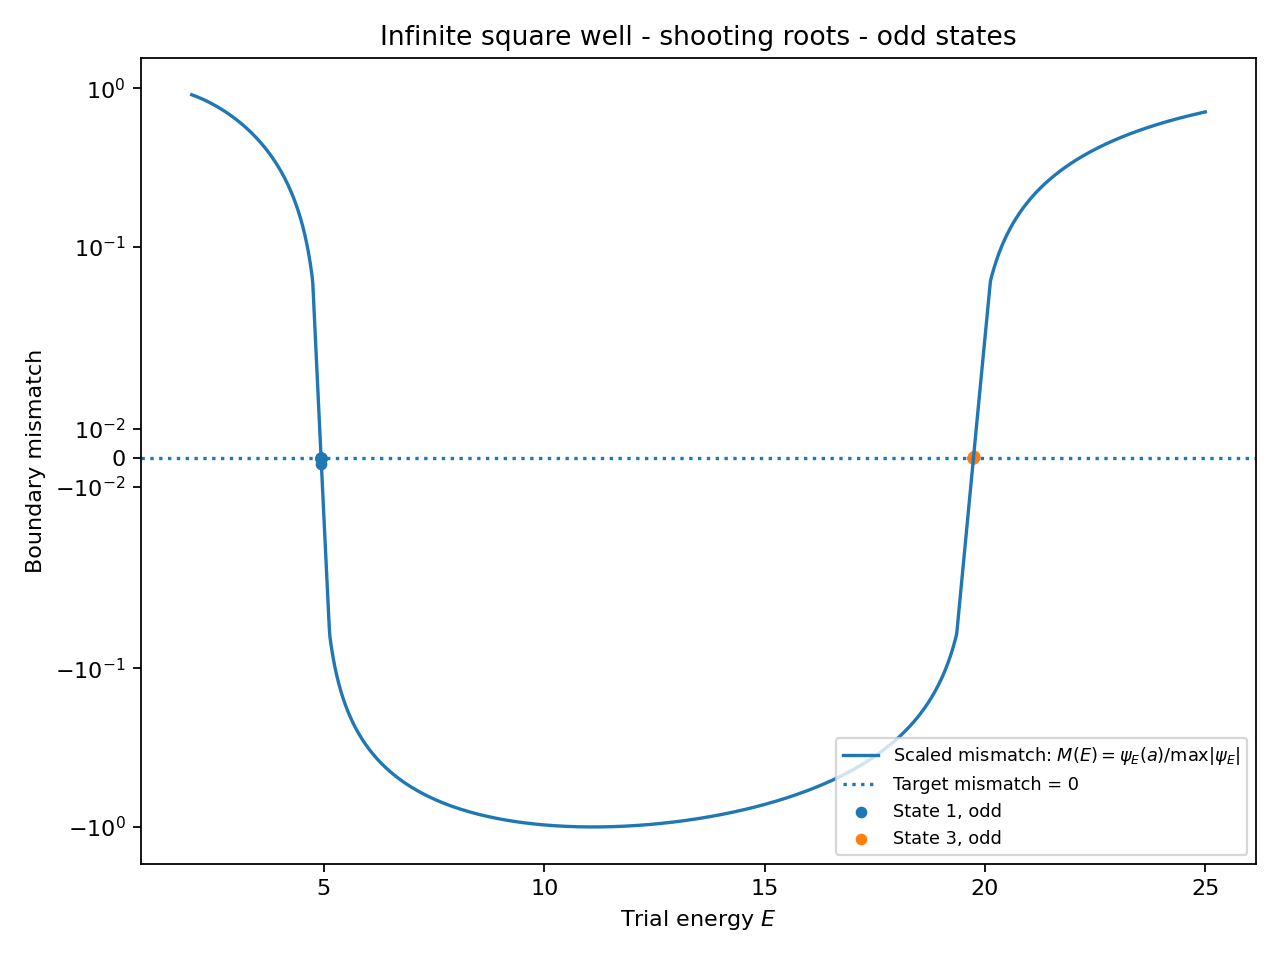
\includegraphics[height=5cm]{../../results/1_infinite_square_well_Numerov/1_infinite_square_well_Numerov_root_finding_odd.png}
                        \caption{}
                    \end{subfigure}

                    \captionof{figure}{Root-finding mismatch function; zeros correspond to eigenvalues.}
                    \label{fig:infwell_shooting}
                \end{minipage}
            \end{figure}

            The infinite square well serves as a benchmark problem with known analytic spectrum:
            \begin{equation}
            E_n = \frac{(n+1)^2\pi^2}{8a^2}
            \end{equation}
            The potential is:
            \begin{equation}
            V(x)=\begin{cases}
            0 & ,|x|\le a\\
            \infty & ,|x|>a
            \end{cases}
            \qquad \text{(implemented numerically with a large finite }V_0\text{)}
            \end{equation}
            In the production calculation, the well half-width is $a=1$, the outward-shooting half-domain uses $x_{\max}=a=1$, the Numerov grid uses $n_{\text{grid}}=2500$ points, and the numerical wall height is set to $V_0=10^6$. A separate grid-refinement study is used to check convergence at fixed $x_{\max}=1$. \\

            The numerical eigenvalues agree with the analytic values to essentially machine precision, as shown in Fig.~\ref{fig:infwell_energies}; in the saved run the first four relative errors are of order $10^{-11}$--$10^{-10}$. Figure~\ref{fig:infwell_states} shows the expected parity and node structure, while Fig.~\ref{fig:infwell_shooting} illustrates the shooting mismatch used to isolate the first four roots. The convergence study in Fig.~\ref{fig:infwell_convergence} gives fitted exponents $p=3.94$, $4.00$, $3.98$, and $4.00$, so this benchmark also confirms the expected fourth-order accuracy. \\

            \begin{figure}[t]
                \centering
                
                \begin{minipage}[t]{0.48\textwidth}
                    \centering
                    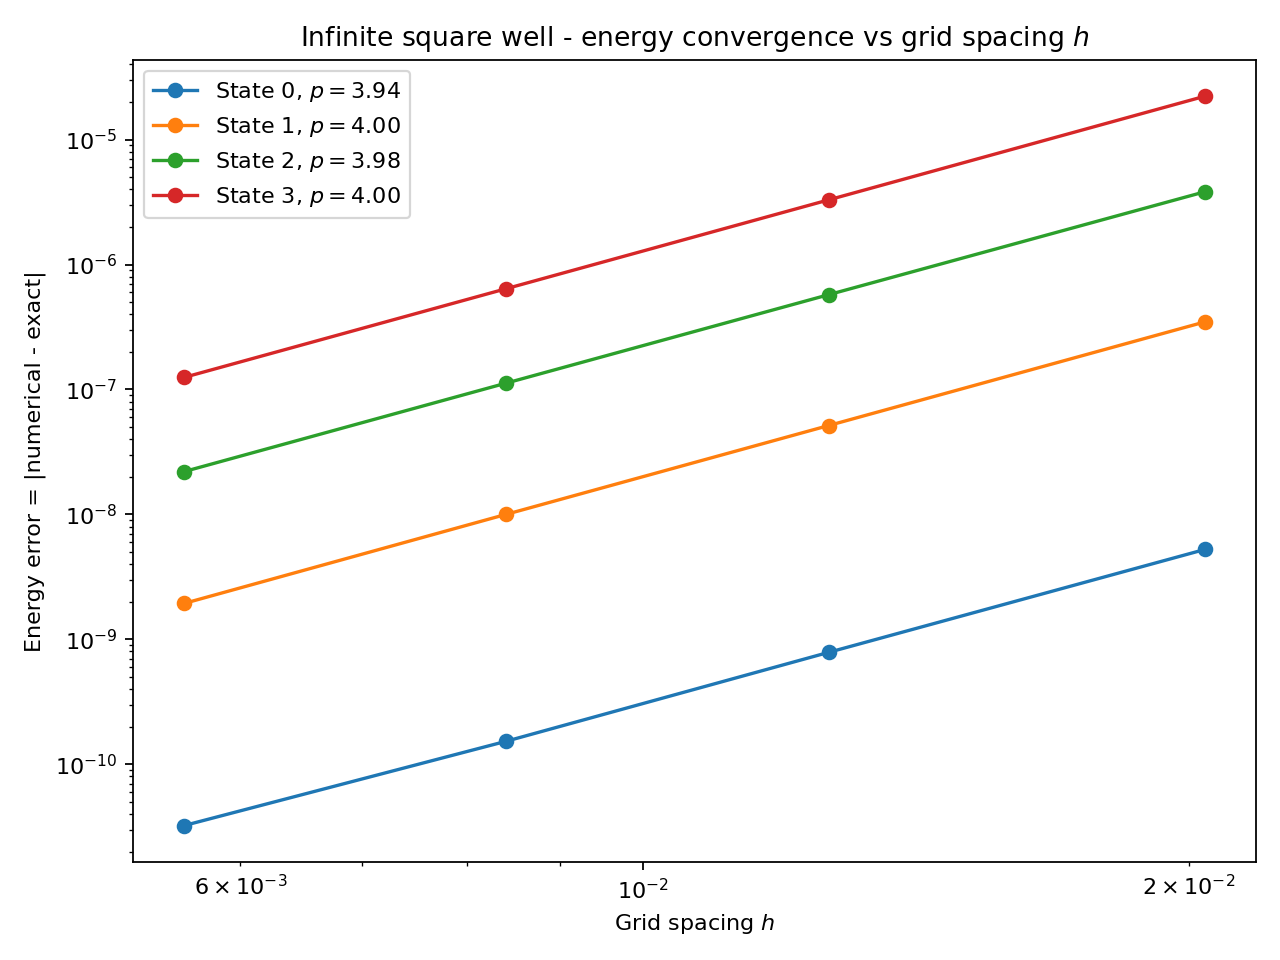
\includegraphics[width=\textwidth]{../../results/1_infinite_square_well_Numerov/1_infinite_square_well_Numerov_energy_convergence_vs_h.png}
                    \captionof{figure}{Energy error versus grid spacing $h$ for the infinite square well.}
                    \label{fig:infwell_convergence}
                \end{minipage}
            \end{figure}

        \subsection{Harmonic oscillator}
            \subsubsection{Numerov method on unbounded domains}
                For the harmonic oscillator with $V(x)=\tfrac{1}{2}\omega^2 x^2$, the exact spectrum is:
                \begin{equation}
                E_n = \omega\left(n+\tfrac{1}{2}\right), \qquad n=0,1,2,\ldots
                \end{equation}
                This provides a second analytic benchmark, but on an unbounded domain. Numerically, the domain is truncated to $[-x_{\max},x_{\max}]$, and decaying boundary conditions are imposed. In the production Numerov run, the parameters are $\omega=1$, $x_{\max}=8$, and $n_{\text{grid}}=2500$. Separate studies vary the grid spacing at fixed $x_{\max}$ and the box size at approximately fixed spacing. \\

                The numerical eigenvalues agree with the exact linear spectrum to extremely high precision, with first-four-state relative errors of order $10^{-12}$--$10^{-11}$ in the saved run. The convergence studies in Figs.~\ref{fig:ho_convergence_h} and \ref{fig:ho_convergence_xmax} quantify the discretization and truncation errors for this unbounded-domain benchmark. \\

                \begin{figure}[!b]
                    \centering

                    \begin{minipage}[t]{0.48\textwidth}
                        \centering
                        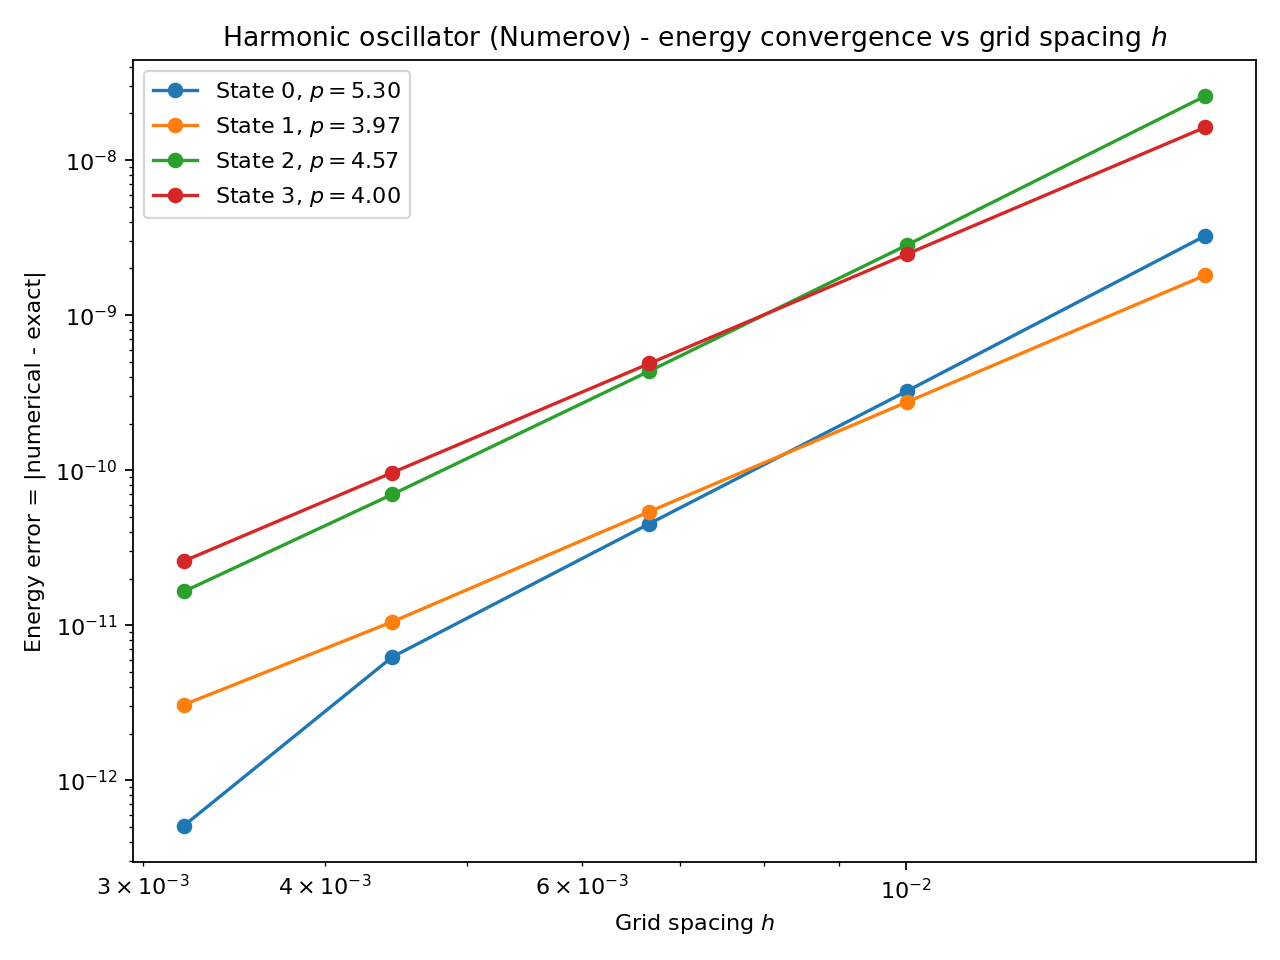
\includegraphics[width=\textwidth]{../../results/2a_harmonic_oscillator_Numerov/2a_harmonic_oscillator_Numerov_energy_convergence_vs_h.png}
                        \captionof{figure}{Energy error versus grid spacing $h$ for the harmonic oscillator.}
                        \label{fig:ho_convergence_h}
                    \end{minipage}
                    \hfill
                    \begin{minipage}[t]{0.48\textwidth}
                        \centering
                        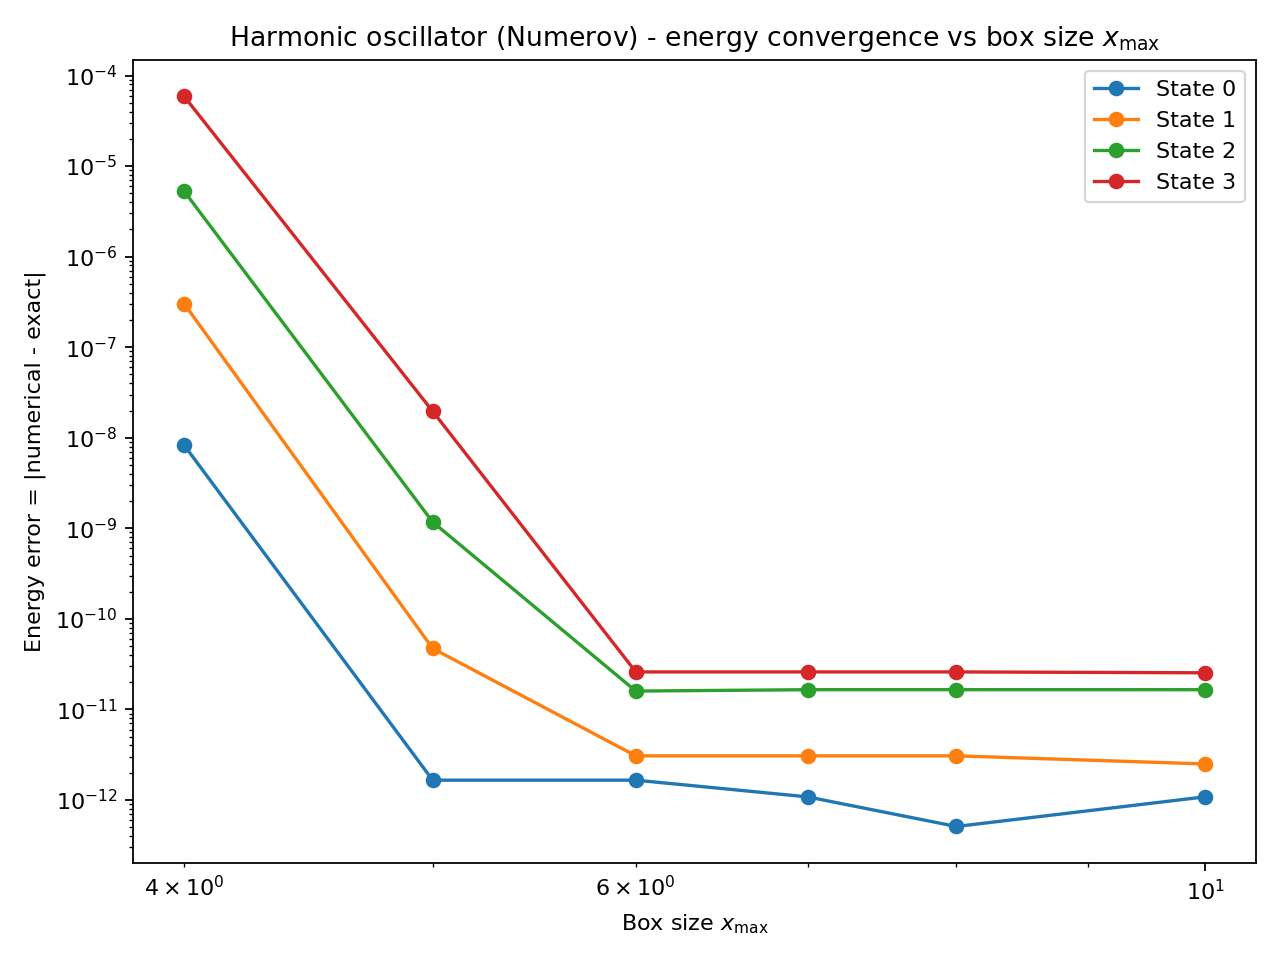
\includegraphics[width=\textwidth]{../../results/2a_harmonic_oscillator_Numerov/2a_harmonic_oscillator_Numerov_energy_convergence_vs_x_max.png}
                        \captionof{figure}{Energy error versus domain size $x_{\max}$ for the harmonic oscillator.}
                        \label{fig:ho_convergence_xmax}
                    \end{minipage}
                \end{figure}

                The convergence study versus grid spacing in Fig.~\ref{fig:ho_convergence_h} is consistent with fourth-order behavior. The saved fits give $p\approx5.30$, $3.97$, $4.57$, and $4.00$ for the first four states; the values above four occur only once the errors are already near the numerical floor and are therefore not interpreted as true superconvergence. The box-size study in Fig.~\ref{fig:ho_convergence_xmax} shows the expected truncation-to-discretization crossover: enlarging the domain rapidly reduces the error at first, after which the curves flatten once truncation error is no longer dominant. \\

            \subsubsection{Numerov versus Runge--Kutta}
                As an additional method comparison, the harmonic oscillator was also solved using a fourth-order Runge--Kutta (RK4) shooting method \cite{Pang_2006}. In this formulation the second-order Schr\"odinger equation is rewritten as the first-order system:
                \begin{equation}
                \psi' = \phi, \qquad
                \phi' = 2[V(x)-E]\psi
                \end{equation}
                This makes RK4 a useful general-purpose comparison for Numerov, which instead exploits the special second-order structure of the Schr\"odinger equation directly. The RK4 comparison uses the same physical parameters $\omega=1$ and $x_{\max}=8$ as the Numerov run, and it reuses the same family of grid spacings derived from the Numerov convergence study so the two methods are compared on matched meshes. \\

                Figure~\ref{fig:ho_numerov_vs_rk4} compares the maximum energy error over the computed harmonic-oscillator states as a function of grid spacing. Both methods show approximately fourth-order convergence, but Numerov gives the smaller error on the matched grids, typically by a factor of about $2$--$4$. The RK4 slopes are also more uniformly close to four, while the Numerov fit is affected more strongly once the errors approach the numerical floor. This comparison is included mainly to show the benefit of using a method specialized to second-order equations when the boundary diagnostics are implemented with comparable care.

                \begin{figure}[!h]
                    \centering

                    \begin{minipage}[t]{0.48\textwidth}
                        \centering
                        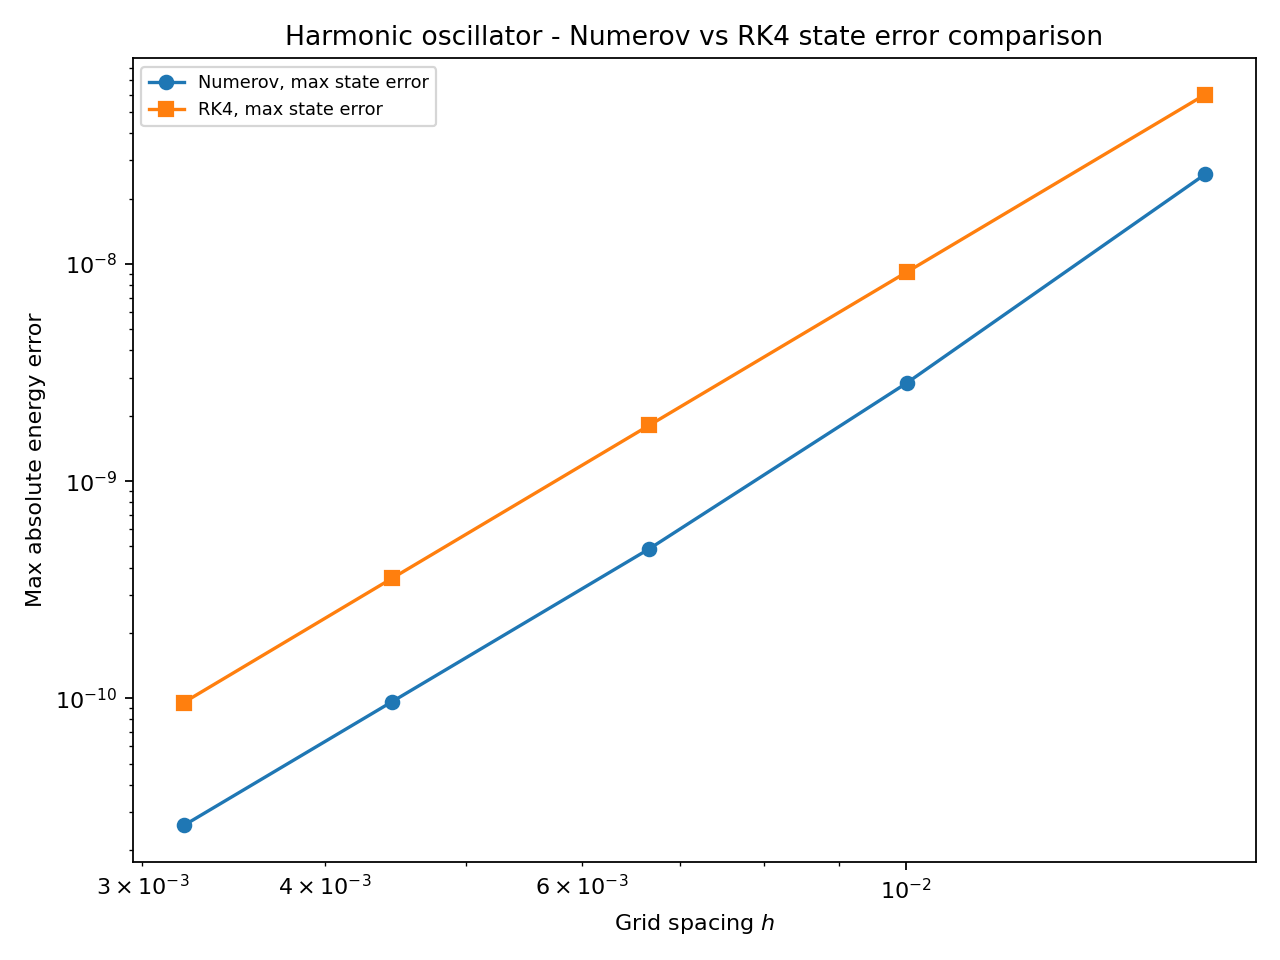
\includegraphics[width=\textwidth]{../../results/2c_harmonic_oscillator_Numerov_VS_RK4_comparison/2c_harmonic_oscillator_Numerov_VS_RK4_state_error_comparison.png}
                        \captionof{figure}{Maximum energy error versus grid spacing for Numerov and RK4.}
                        \label{fig:ho_numerov_vs_rk4}
                    \end{minipage}
                \end{figure}

        \subsection{Double-well potential}
            The quartic double-well potential is used as the main nontrivial bound-state example. In the shifted form used here:
            \begin{equation}
            V(x)=ax^4-bx^2-V_{\min}, \qquad V_{\min}=-\frac{b^2}{4a}
            \end{equation}
            the two minima are shifted to zero. This shift is applied using the analytic minimum $V_{\min}=-b^2/{4a}$ rather than the sampled grid minimum $\min_i(V(x_i))$ taken over the current mesh points, because the sampled minimum drifts slightly as the grid changes and would otherwise contaminate convergence studies. The analytic shift also gives a cleaner energy reference: the well bottoms sit at zero, so the reported low-lying energies can be read directly relative to the bottoms of the wells, while the potential shape and tunneling splittings remain unchanged. Unlike the infinite square well and harmonic oscillator, this system does not have a simple analytic spectrum, so the validation relies on internal consistency checks, convergence studies, parity structure, and physically expected tunneling behavior. The production run uses $a=1$, $b=6$, the analytic minimum shift $V_{\min}=-b^2/{4a}$, a box size $x_{\max}=4$, and $n_{\text{grid}}=4000$. Separate studies are used to test grid refinement, box-size sensitivity, and the dependence of the lowest splitting on the parameter $b$. \\

            Figure~\ref{fig:dw_states} shows the first four computed states together with the double-well potential. The lowest two form a nearly degenerate even-odd pair, $E_0\approx2.357273$ and $E_1\approx2.359372$, with a splitting of about $2.10\times10^{-3}$; the next pair, $E_2\approx6.548814$ and $E_3\approx6.684430$, is more strongly split. \\

            Since no closed-form spectrum is available, grid convergence is measured through successive refinements at fixed domain size using the surrogate error $|E(h_i)-E(h_{i+1})|$. Figure~\ref{fig:dw_splitting} shows the main physical trend of the section: as $b$ increases from $3$ to $8$, the lowest even-odd splitting falls from about $3.52\times10^{-1}$ to $1.59\times10^{-5}$, indicating tunneling suppression as the wells deepen and separate. \\

            \begin{figure}[h]
                \centering

                \begin{minipage}[t]{0.48\textwidth}
                    \centering
                    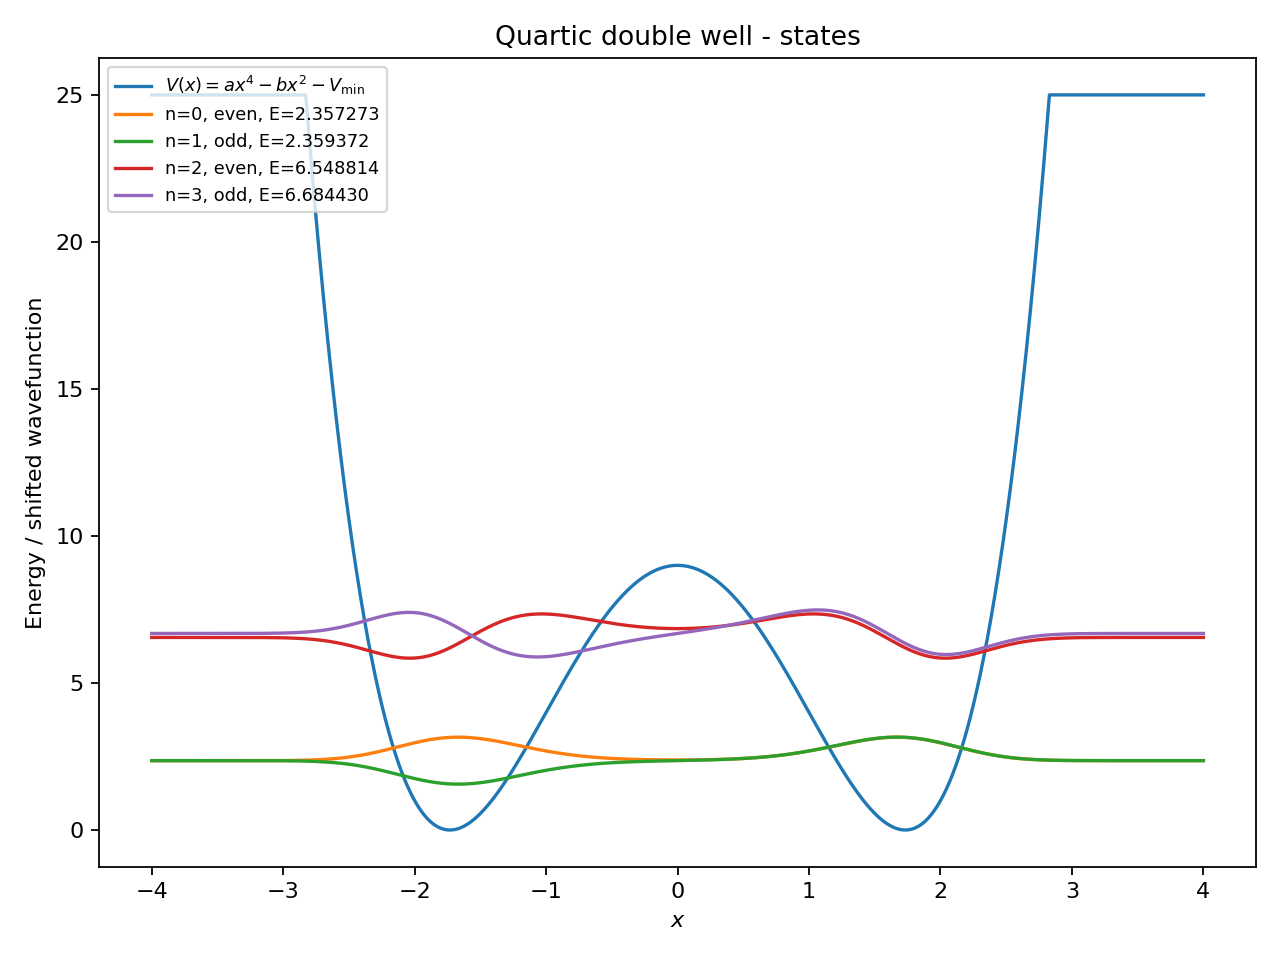
\includegraphics[width=\textwidth]{../../results/3_double_well_Numerov/3_double_well_Numerov_states.png}
                    \captionof{figure}{First four bound states of the quartic double-well potential.}
                    \label{fig:dw_states}
                \end{minipage}
                \hfill
                \begin{minipage}[t]{0.48\textwidth}
                    \centering
                    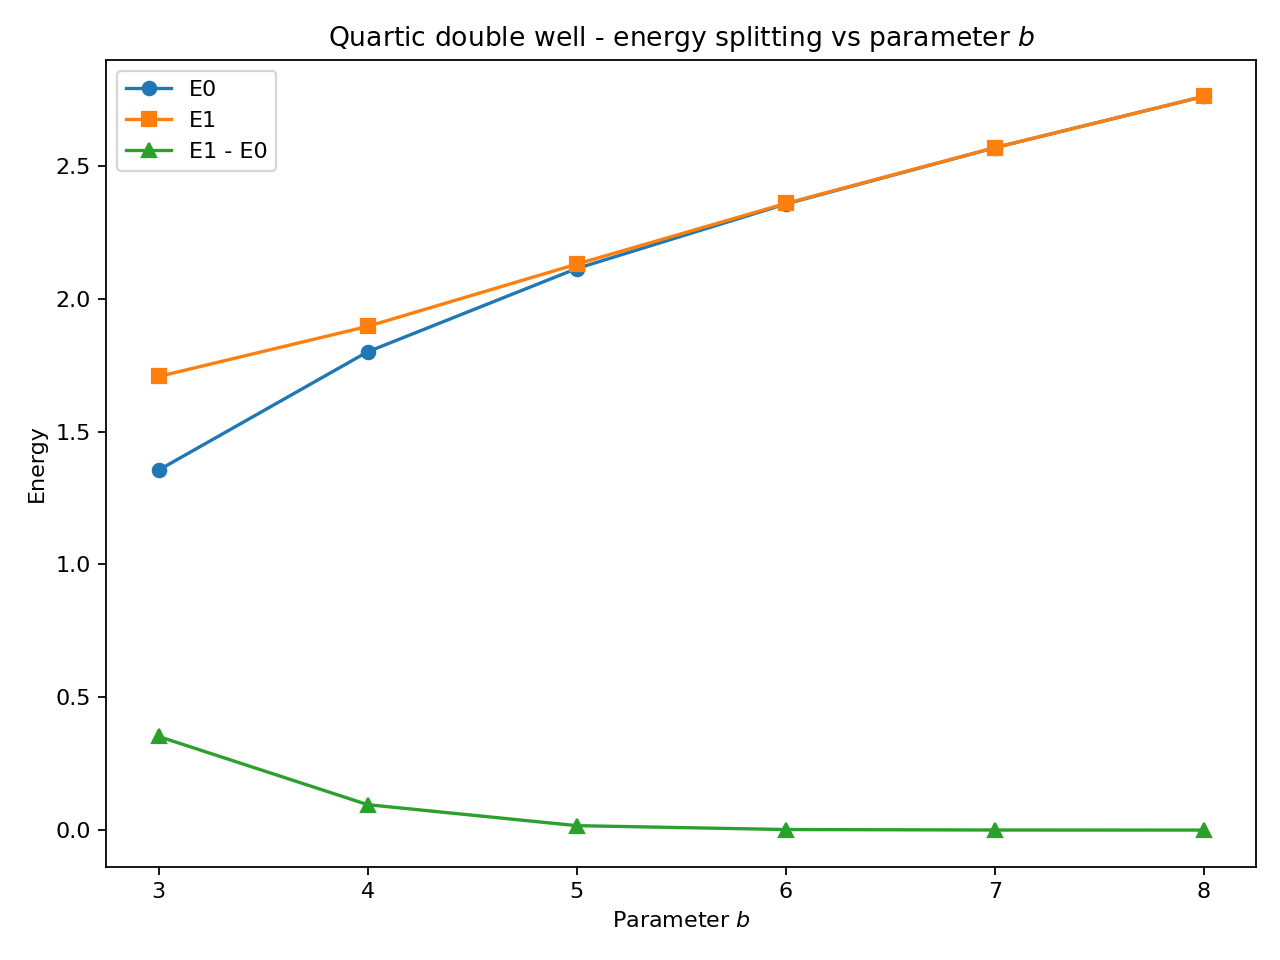
\includegraphics[width=\textwidth]{../../results/3_double_well_Numerov/3_double_well_Numerov_energy_splitting_vs_b.png}
                    \captionof{figure}{Lowest two double-well energies and their splitting versus $b$.}
                    \label{fig:dw_splitting}
                \end{minipage}
            \end{figure}

        \subsection{Finite square well}
            The finite square well is included as an additional nontrivial bound-state test. Unlike the infinite square well, the potential walls are finite, so bound states can leak into the classically forbidden region. The potential used here has the form:
            \begin{equation}
            V(x)=\begin{cases}
            0 & ,|x|\le a\\
            V_0 & ,|x|>a
            \end{cases}
            \end{equation}
            and only states with $E<V_0$ are true bound states. In the production run, the well parameters are $a=1$ and $V_0=12$, while the outward-shooting box uses $x_{\max}=4$ and the Numerov mesh uses $n_{\text{grid}}=3000$. A supplementary grid-refinement check compares coarser solutions to the finest saved run, so the plotted quantity is $|E_N-E_{\mathrm{ref}}|$ with the $n_{\text{grid}}=3000$ spectrum acting as the practical reference. Unlike the smooth benchmark potentials, however, the finite square well is only piecewise smooth: $V(x)$ jumps at $|x|=a$. That discontinuity degrades the observed asymptotic convergence order, so this refinement study should be read mainly as a practical convergence check rather than a clean fourth-order Numerov benchmark. \\

            Figure~\ref{fig:finitewell_states} shows the first four computed states together with the finite well potential. For $V_0=12$ and $a=1$, the first three states are well localized inside the well, while the fourth lies close to the barrier top and shows much stronger leakage into the exterior region. \\

            As $E\to V_0^{-}$, the exterior decay constant tends to zero, so near-threshold states are the most sensitive part of the finite-well spectrum. The grid-refinement study is included mainly as a practical convergence check, since the discontinuity at the well edge lowers the observed asymptotic order relative to the smooth benchmark cases. \\

            \begin{figure}[h]
                \centering

                \begin{minipage}[t]{0.48\textwidth}
                    \centering
                    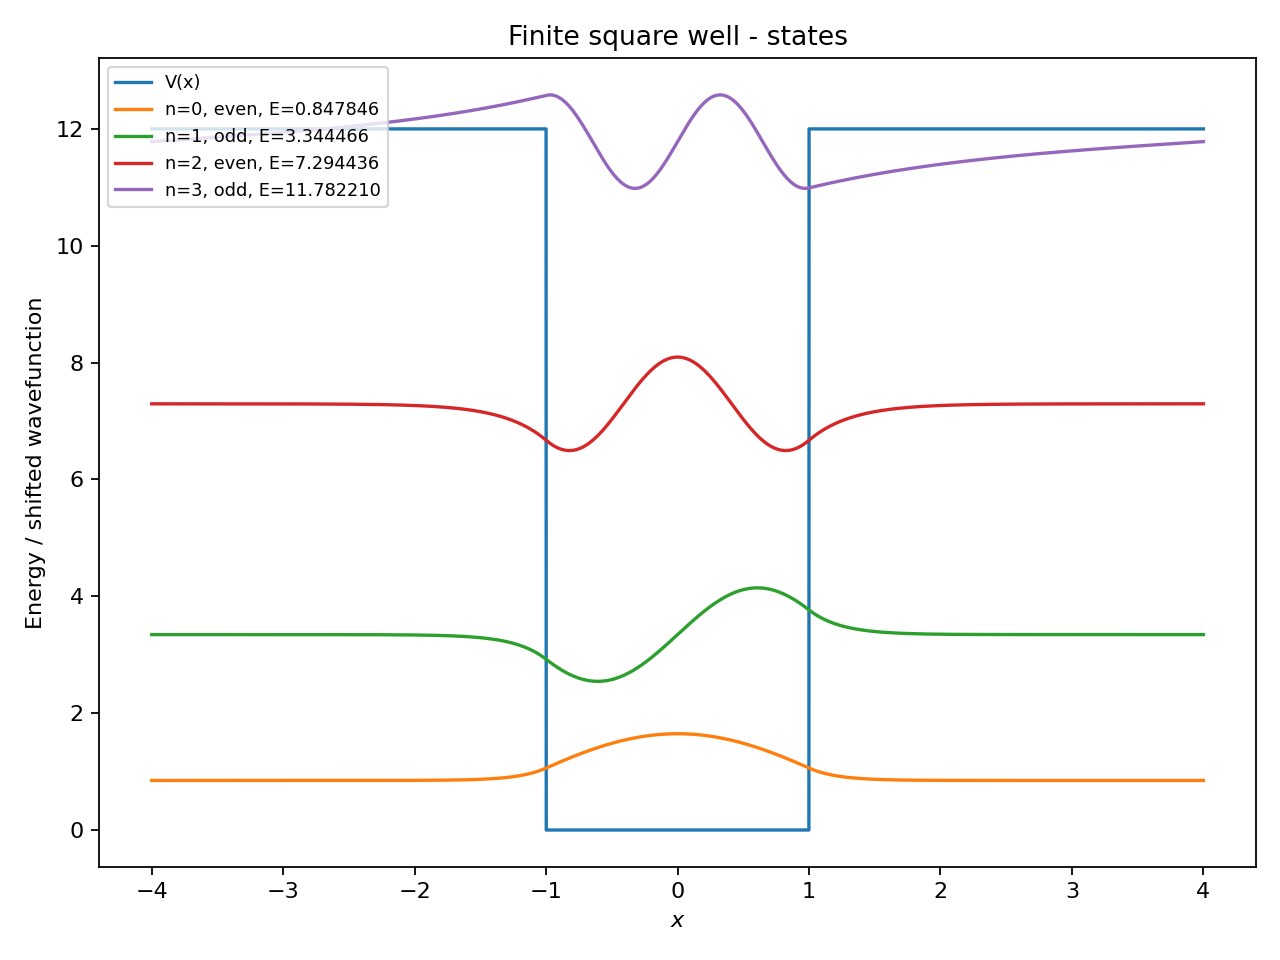
\includegraphics[width=\textwidth]{../../results/4_finite_square_well_Numerov/4_finite_square_well_Numerov_states.png}
                    \captionof{figure}{First four finite-square-well states and the finite barrier potential.}
                    \label{fig:finitewell_states}
                \end{minipage}
            \end{figure}

        \subsection{Scattering and resonant tunneling}
            \subsubsection{Single barrier potential}
                As a secondary extension beyond bound states, the Numerov framework is also applied to one-dimensional scattering from a finite rectangular barrier. For each incident energy $E$, the complex wavefunction is propagated through the barrier region and decomposed into incident, reflected, and transmitted waves. This gives the transmission and reflection probabilities $T(E)$ and $R(E)$. The integration is started from the right free region, not the left, because the right boundary condition is the simplest one to impose directly: for a left-incident scattering state, the far-right asymptotic solution contains only the transmitted outgoing wave $e^{ikx}$. The left asymptotic region is more complicated because it contains a superposition of incident and reflected waves, so those amplitudes are recovered afterward by decomposing the numerically propagated left solution. \\

                The shared scattering grid for both barrier problems is $x\in[-8,8]$ with $n_{\text{grid}}=4000$ points. For the single-barrier run, the barrier parameters are $V_0=5$, width $1.2$, and center $0$, while the incident energy is scanned over a range that covers both below-barrier and above-barrier behavior. \\

                The single-barrier result is shown in Fig.~\ref{fig:single_barrier_scattering}. Transmission is strongly suppressed at low incident energy and increases as the energy rises through and above the barrier. Even for $E>V_0$, transmission is not exactly one because the finite interfaces still cause partial reflection. The conservation check $T(E)+R(E)$ remains numerically indistinguishable from one across the saved scan. \\

                \begin{figure}[h]
                    \centering

                    \begin{minipage}[t]{0.48\textwidth}
                        \centering
                        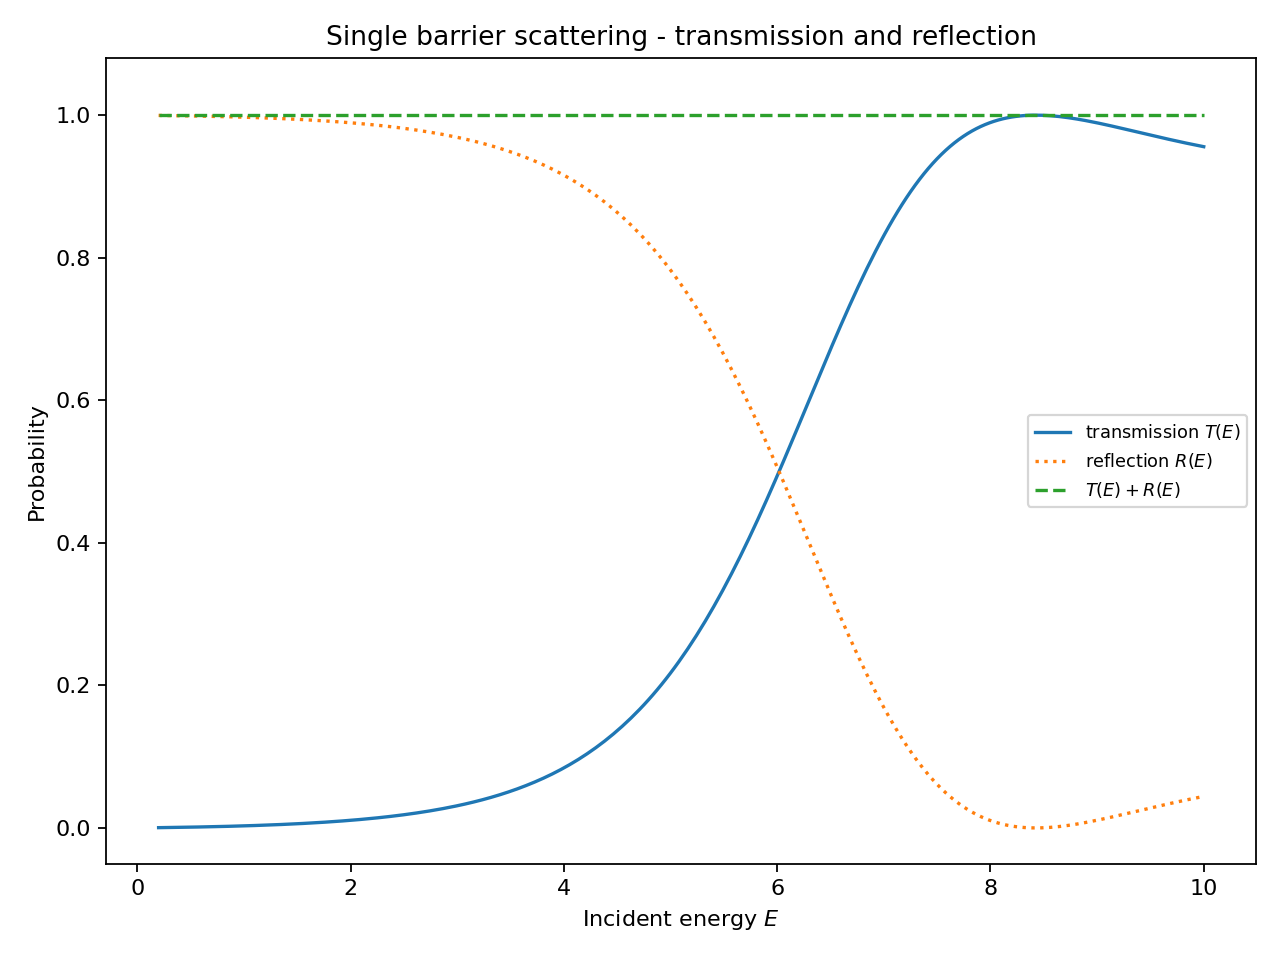
\includegraphics[height=5cm]{../../results/5_scattering_single_barrier_Numerov/5_scattering_single_barrier_Numerov_transmission_reflection.png}
                        \caption{Transmission and reflection probabilities for a finite rectangular barrier.}
                        \label{fig:single_barrier_scattering}
                    \end{minipage}
                \end{figure}

            \subsubsection{Double barrier potential}
                The double-barrier potential is used to demonstrate resonant tunneling. In this case the two barriers create an intermediate well, so certain incident energies can form quasi-bound states between the barriers. At these energies, destructive reflection and constructive transmission lead to sharp peaks in the transmission coefficient. \\

                For the production double-barrier run, each barrier has height $V_0=5$, the barrier width is $0.6$, the central well width is $1.4$, the structure is centered at $x=0$, and the incident energy is scanned across the resonance region below the barrier top. Resonance candidates are then identified from peaks in the transmission curve. \\

                Figure~\ref{fig:double_barrier_resonances} shows two clear resonances in the saved transmission curve: a narrow low-energy peak near $E\approx1.13938$ and a broader high-energy peak near $E\approx4.35847$, both with transmission very close to one. The conservation check $T(E)+R(E)$ remains essentially exact across the scan. Figure~\ref{fig:double_barrier_resonant_state} shows the probability density at the first resonance, where the wavefunction is strongly enhanced in the region between the barriers, identifying the quasi-bound state responsible for resonant tunneling. \\

                \begin{figure}[h]
                    \centering

                    \begin{minipage}[t]{0.48\textwidth}
                        \centering
                        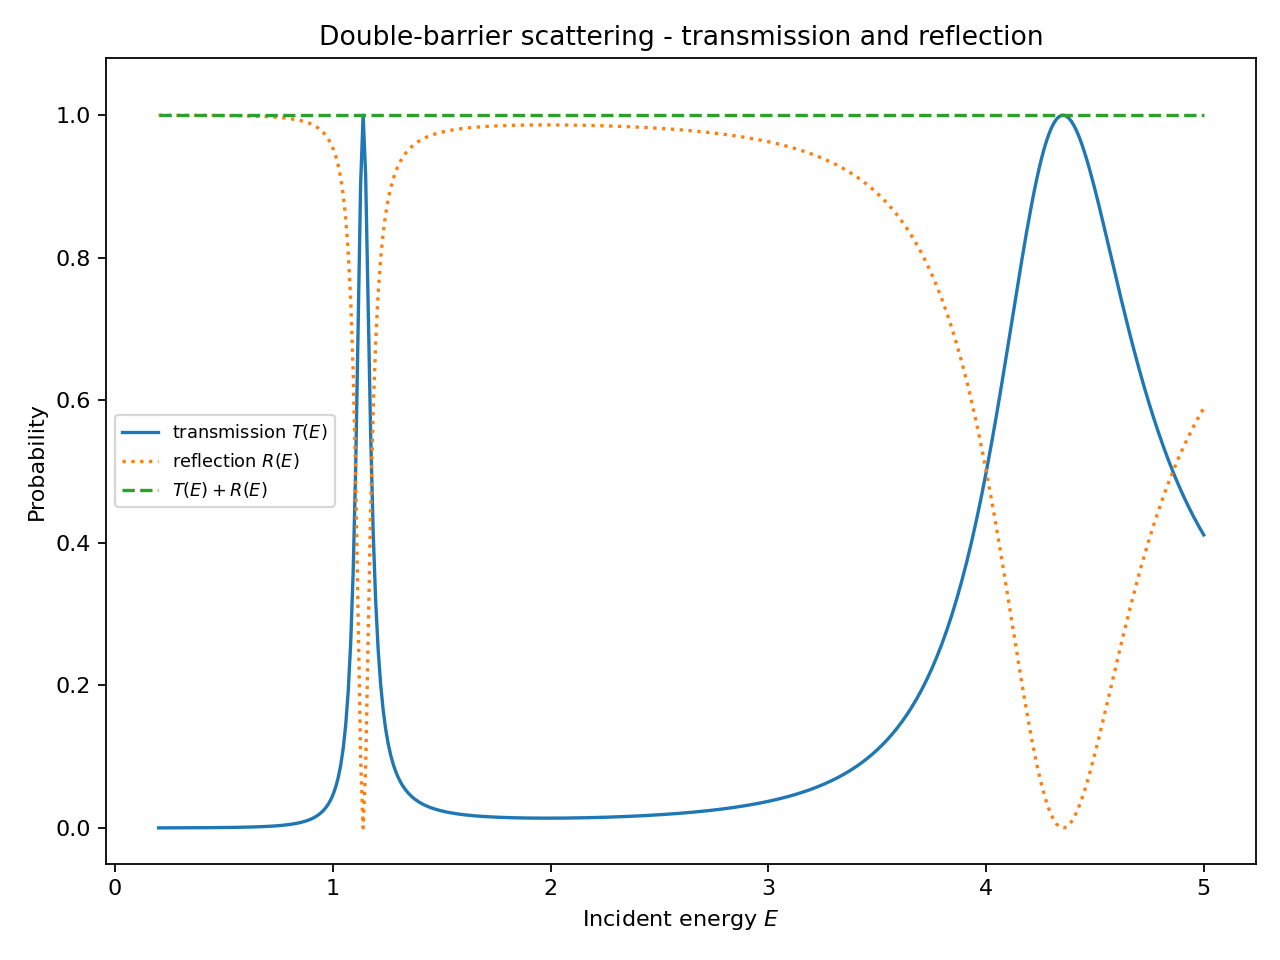
\includegraphics[width=\textwidth]{../../results/6_scattering_double_barrier_Numerov/6_scattering_double_barrier_Numerov_transmission_reflection.png}
                        \captionof{figure}{Transmission and reflection probabilities for the double-barrier potential.}
                        \label{fig:double_barrier_resonances}
                    \end{minipage}
                    \hfill
                    \begin{minipage}[t]{0.48\textwidth}
                        \centering
                        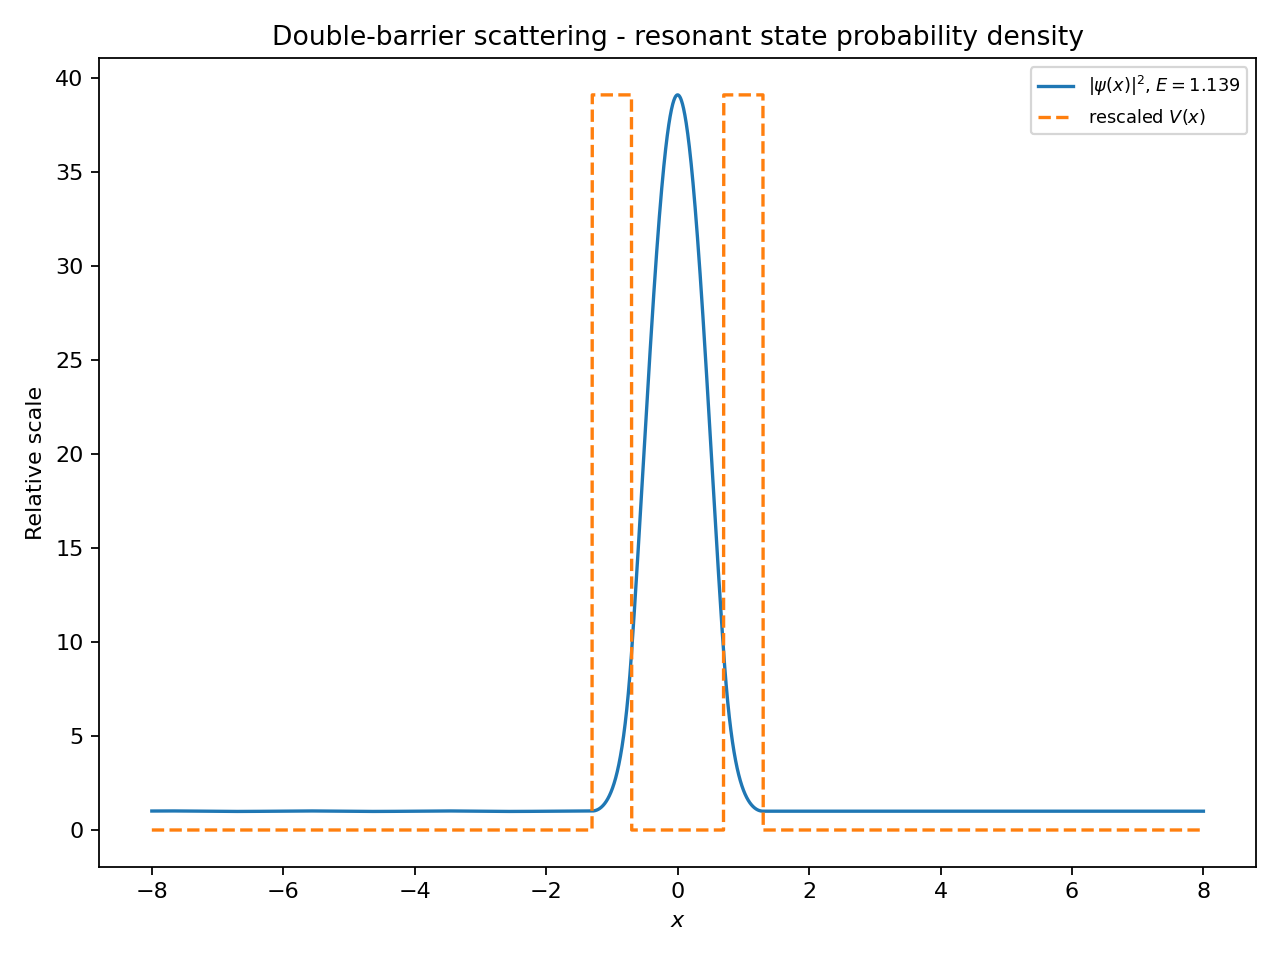
\includegraphics[width=\textwidth]{../../results/6_scattering_double_barrier_Numerov/6_scattering_double_barrier_Numerov_state_probability_density.png}
                        \captionof{figure}{Probability density at the first resonant energy.}
                        \label{fig:double_barrier_resonant_state}
                    \end{minipage}
                \end{figure}

    % ==============================================================
    % Discussion
    % ==============================================================
    \section{Discussion}
        The calculation was checked in four complementary ways: automated tests of key numerical components, analytic benchmark spectra for the infinite square well and harmonic oscillator, inspection of parity and node structure in the wavefunctions, and convergence studies with respect to both grid spacing and domain size. Taken together, these checks show that the method is reliable when the boundary treatment is handled with the same care as the integration formula itself. \\

        The convergence studies also identify the main practical limitations. In the smooth benchmark problems, the observed behavior is consistent with fourth-order accuracy, while slopes slightly above four occur only once the errors are already near the numerical floor. The harmonic-oscillator box-size study separates domain truncation from discretization error, and the RK4 comparison shows that method order alone is not enough: once the inward boundary derivative is evaluated accurately, Numerov gives smaller errors than RK4 at matched grid spacing. For the quartic double well, where no exact spectrum is available, correctness is established through self-consistency, parity-separated diagnostics, and stable refinement behavior. The finite well and scattering extensions show that the same framework also handles barrier penetration and resonant tunneling without losing flux conservation or qualitative physical consistency. \\

    % ==============================================================
    % Conclusion
    % ==============================================================
    \section{Conclusion}
        This project implemented a Numerov shooting solver for the one-dimensional time-independent Schr\"odinger equation and validated it on analytic benchmark problems. The method recovers the infinite-well and harmonic-oscillator spectra to very high precision and shows the expected high-order convergence when the boundary treatment is implemented consistently. \\

        The same framework also resolves nontrivial physics beyond the benchmarks, including tunneling splitting in a quartic double well, barrier penetration in a finite square well, and resonant transmission through double barriers. Overall, the results show that Numerov shooting is an accurate and flexible method for one-dimensional quantum calculations when boundary diagnostics and convergence checks are treated as part of the numerical method itself.

    % ==============================================================
    % References
    % ==============================================================
    \printbibliography[heading=bibintoc,title={References}]
    \end{refsection}
\end{document}
